\section{Web Server}
Socket programming (TCP/IP)을 통해서 web server를 구현했다.

\subsection{Code}
\vspace{-4mm}
\begin{listing}[h!]
\inputminted[framerule = 1pt,framesep = 2mm , frame = lines, fontsize=\footnotesize]{python}{./code/week09/01/server.py}
\caption{\footnotesize Experiment 1, server.py}
\end{listing}
\clearpage

\subsection{Process Analysis}
\begin{enumerate}
    \item TCP/IP Server socket 생성(socket) 및 IP 주소와 Port 번호 설정(bind)
    \item Server가 Client로부터 연결 요청이 있는지 수신 대기(listen)
    \item Server가 Client의 연결 요청을 수락(accept)
    \item Server가 Client로부터 HTTP request message 수신(recv)
    \item Server는 Client가 요청한 HelloWorld.html 파일을 읽어 buffer에 저장
    \item Server는 Client에게 요청이 성공했음을 알리는 ‘HTTP/1.1 200 OK’ HTTP response header line 송신(send)
    \item Server가 Client에게 HelloWorld.html 파일 한 글자씩 전송(send)
    \item Server/Client socket close으로 TCP connection 종료
\end{enumerate}

\subsection{Experiment Result}
Webserver.py와 같은 경로에 HelloWorld.html 파일을 넣고 Web server를 실행했다. \\
\vspace{-4mm}
\begin{figure}[!h]\centering 
	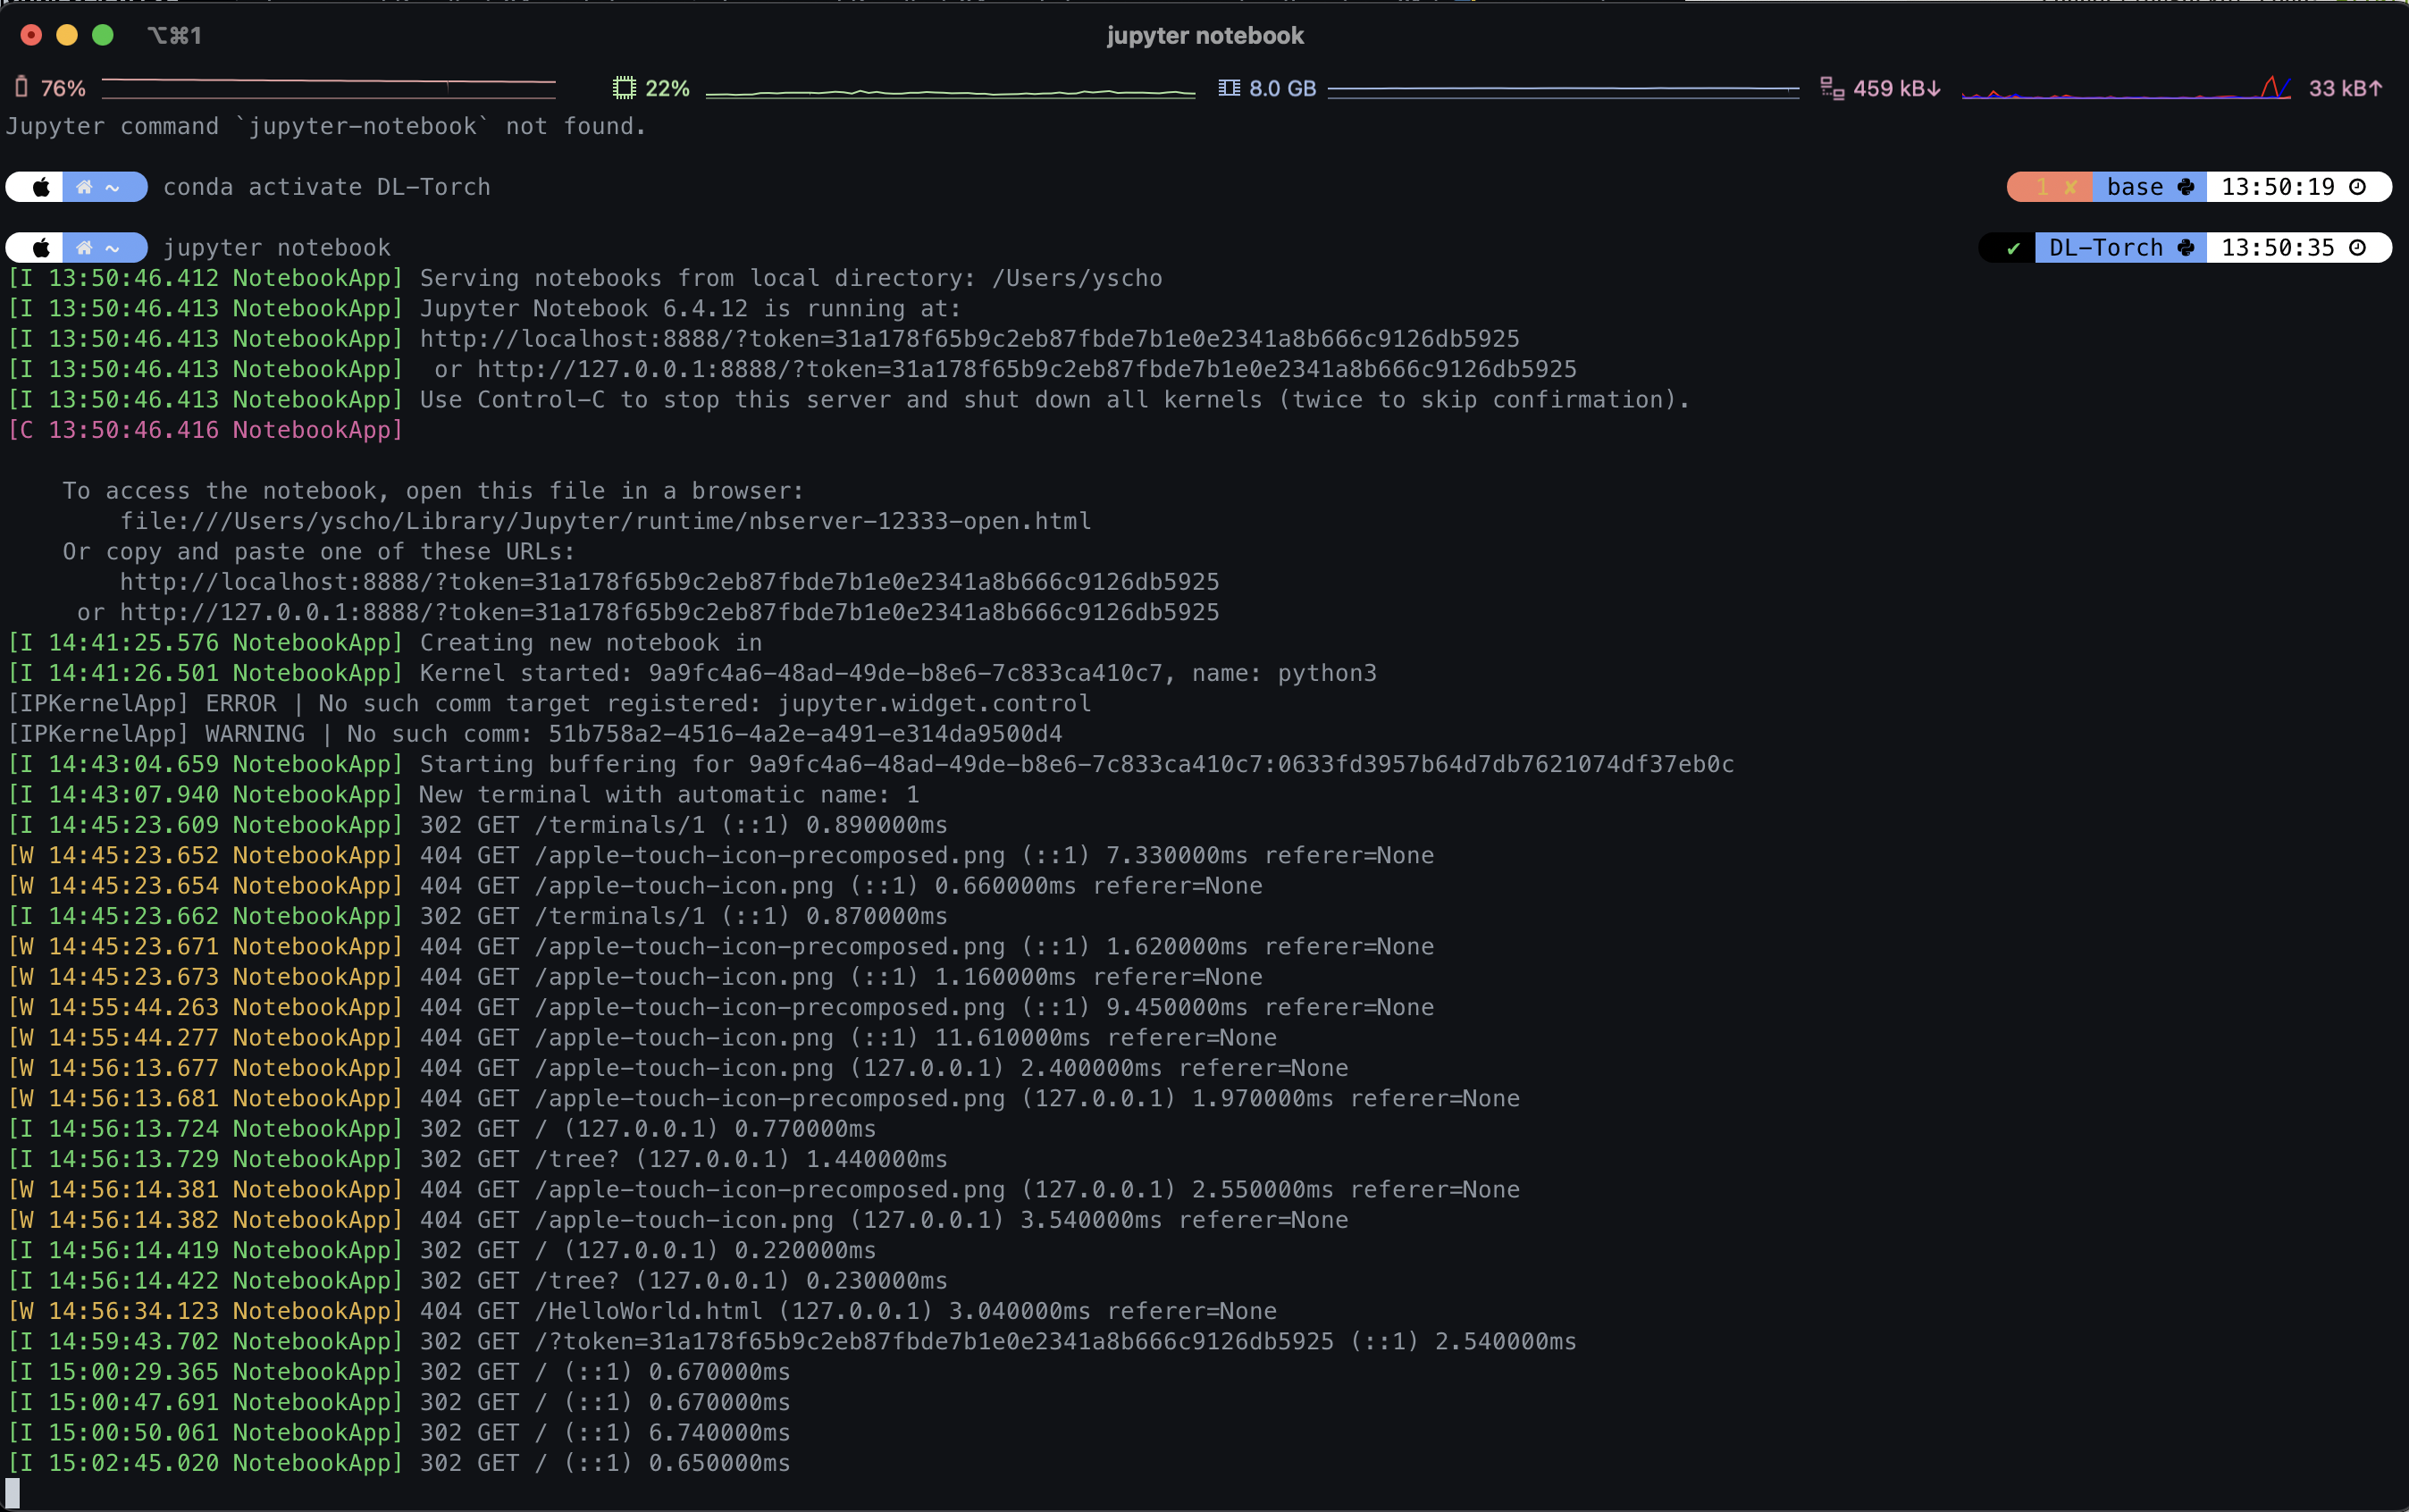
\includegraphics[width=.99\textwidth]{image/week09/1-1.png}
	\caption{\footnotesize
	Executing Web server}
	\vspace{-10pt}
\end{figure}
\clearpage

웹 브라우저에 서버의 IP 주소, 포트, 파일이름 localhost:6789/HelloWorld.html을 입력하여 서버안에 있는 파일인 HelloWorld.html에 접근했다. \\
\vspace{-4mm}
\begin{figure}[!h]\centering 
	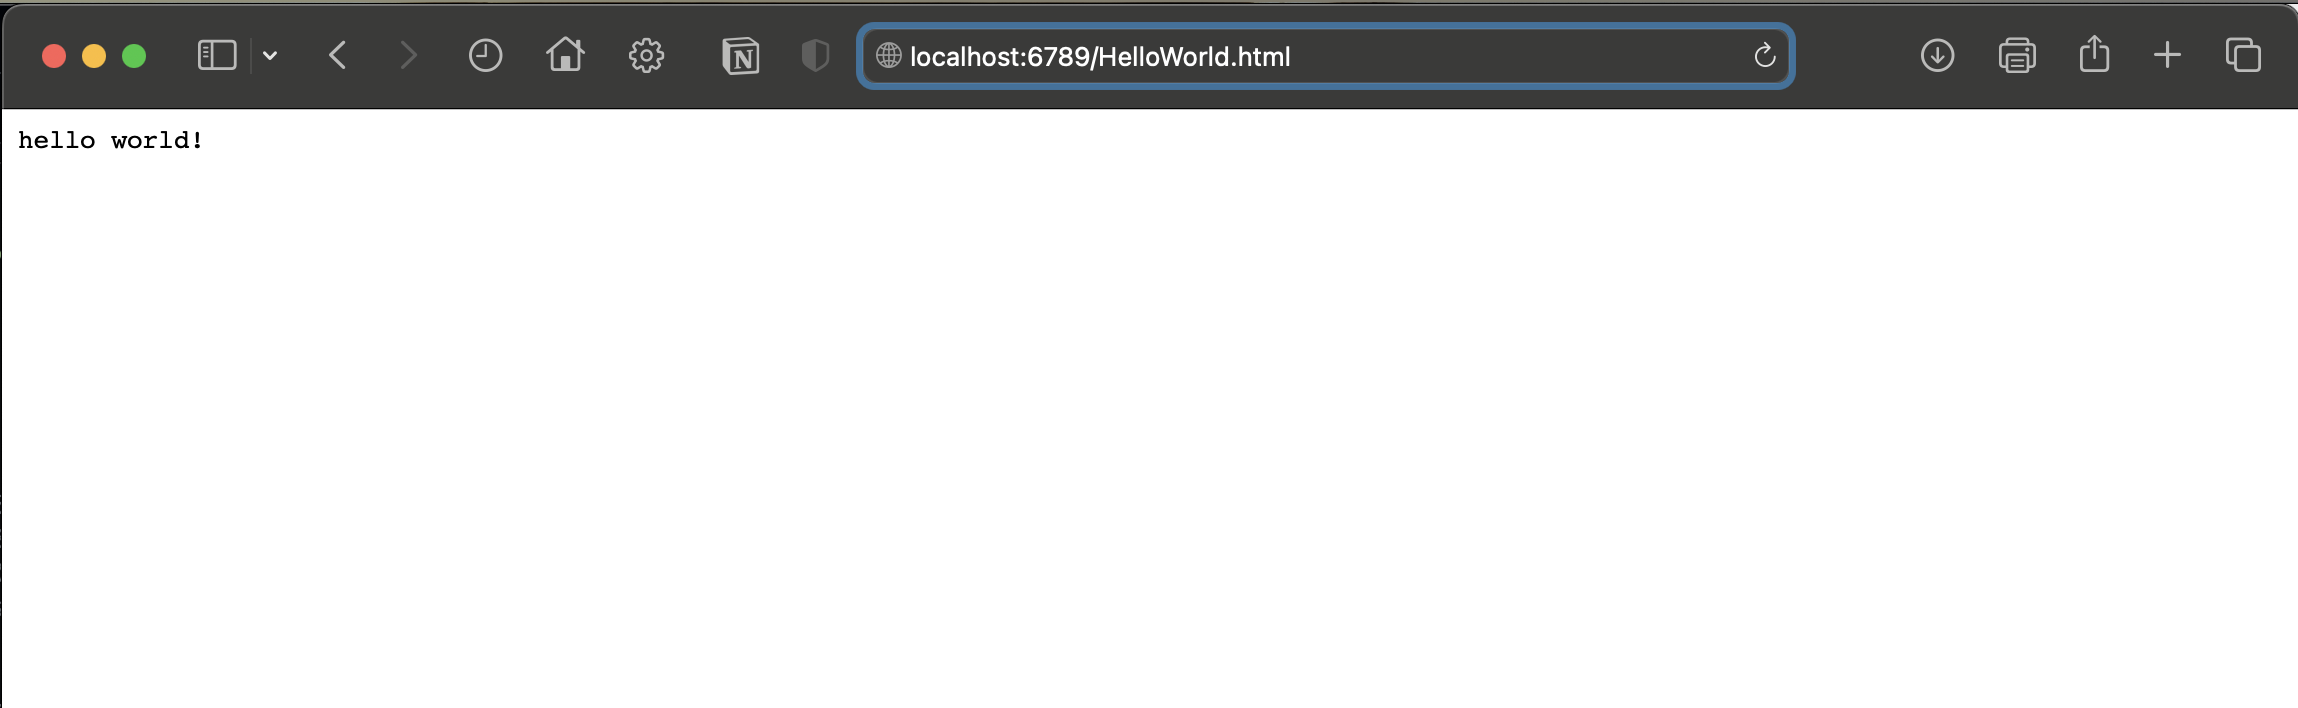
\includegraphics[width=.99\textwidth]{image/week09/1-2.png}
	\caption{\footnotesize
	Web browser accessing HelloWorld.html}
	\vspace{-10pt}
\end{figure}

\clearpage

